% !Mode:: "TeX:UTF-8"
\chapter{Practice: Stereo Visual SLAM}
\begin{mdframed}  
	\textit{Goal of Study}
	\begin{enumerate}[labelindent=0em,leftmargin=1.5em]
	\item Implement a stereo visual SLAM from scratch.
	\item Understand the problems that are prone to occur in VO and how to fix them.
	\end{enumerate}
\end{mdframed}

This lecture is the concluding part of the book. We will use the knowledge we learned before to actually write a visual odometry program. You will manage local robot trajectories and landmarks and experience how a software framework is composed. During the operation, we will encounter many practical problems: how to continuously track the image, control the scale of BA, and so on. To make the program run stably, we need to deal with the above situations, which will bring about many useful discussions on engineering realization.

\newpage
\section{Why do We Have a Separate Engineering Chapter?}
Knowing the principles of bricks and cement does not mean that you can build a grand palace.

In the Minecraft game, all the players have are some blocks with different colors and textures. All the player needs to do is place these blocks on a plane and stack them together. Understanding a block is also extremely simple, but most beginners can only make simple matchbox houses when really starting to build the architectures. Experienced and creative players can use these simple blocks to build houses, gardens, terraces, and pavilions, even the big cities (\autoref{fig:mcarchitecture}~) \footnote{The lower left is my practice work. The bottom right is from the work of the Epicwork team: "Old Summer Palace." I used to study in Epicwork for a while. The creativity of the young people and even the children there left a deep impression on me. }.

\begin{figure}[!htp]
	\centering    
	\includegraphics[width=0.9\linewidth]{designVO/mcarchitecture}\\
	\caption{Great work normally starts from simple things.}
	\label{fig:mcarchitecture}
\end{figure}

In SLAM, we believe that engineering implementation and understanding of algorithm principles should be at least the same important, or even more, as the algorithm principles. The algorithms are like blocks in the building. We can discuss their properties clearly, but just understanding the basic units will not enable you to build an entire building. They require a lot of trials, time, and experience. We encourage readers to work in a more practical direction. Of course, this is often very complicated. Just like in Minecraft, you need to master the structure of various columns, walls, and roofs, wall carvings, and calculation of geometric angles. There are far more contents than discussing the nature of each block.

The same is true for the specific implementation of SLAM. A practical program has a lot of engineering design and skills (tricks), and it is necessary to discuss how to deal with problems after each step. In principle, each SLAM implementation is different. Most of the time, we cannot say which implementation method is the best. However, we usually encounter some common problems like managing map points, dealing with mismatches, selecting keyframes, and so on. We hope that readers can have some intuitive feelings about these possible problems. We think this feeling is vital.

Therefore, out of the emphasis on practice, in this lecture, we will lead the readers through the process of building a SLAM framework. Just like the architecture, we have to discuss trivial but essential issues such as column spacing and facade aspect ratio. SLAM engineering is complicated. Even if we only keep the core part, it will take up a lot of space and make this book too verbose. However, please note that although the final completed project may be complicated, the process of being simple to complex is worthy of detailed discussion. Therefore, we have to start from a simple data structure first, make simple visual odometry, and then slowly add some additional functions. 

The code for this lecture is in \textit{slambook2/ch13}. We will implement a simplified version of stereo VO and then see its running effect in the Kitti dataset. This VO consists of a frontend of optical flow tracking and a backend of sliding window BA. Why choose stereo VO? One reason is that the stereo vision is relatively simple to implement, and initialization can be completed in a single frame. The second is that the stereo camera has 3D observation, and the realization effect will be better than that of the monocular.

\section{Framework}
We are discussing a project realization, and the project usually has the concept of a framework. Most Linux libraries will classify and store algorithm code files according to modules. For example, the header files will be placed in the header file directory, and the source code will be placed in the source code directory. Also, there may be configuration files, test files, third-party libraries, and so on. Now we come to classify our files according to the common practice of small algorithm libraries:

\begin{enumerate}
	\item \textit{bin} stores the compiled binary file;
	\item \textit{include/myslam} stores the header files of the SLAM module. 
	\item \textit{src} stores the source code files, mainly .cpp files.
	\item \textit{test} stores the files used for testing, which are also .cpp files.
	\item \textit{config} stores the configuration files.
	\item \textit{cmake\_modules} saves the cmake files of third-party libraries, which are used by libraries such as g2o.
\end{enumerate}

In this way, we have determined the location of the code file. Now let's discuss the basic data structure involved in VO.

\subsection{Data Structure}
Before writing code, we should clarify what we want to write. A long time ago, there was a classic sentence that \textit{a program is data structure plus algorithm}. For VO, we have to ask: What kind of data does VO need to process? What are the critical algorithms involved? What is the relationship between them?

\begin{itemize}
	\item The most basic unit we deal with is the image. In stereo VO, that is a pair of images. We might as well call it a \textit{frame}.
	\item We will detect visual \textit{features} on the frame. These features are many 2D pixels.
	\item We look for the association of features between images. If we see a feature multiple times, we use the triangulation method to calculate its 3D position, which forms the \textit{landmarks or map points}.
\end{itemize}

Obviously, \textit{images}, \textit{features}, and \textit{landmarks} are the most basic elements in our system. The relationship between them is shown in \autoref{fig:frame-feature-landmark}. In the following description, we use terms landmarks and map points for points in 3D space, and their semantics are the same.

\begin{figure}[!htp]
	\centering
	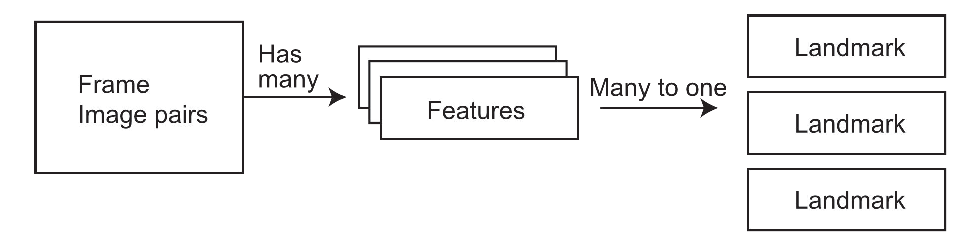
\includegraphics[width=1.0\linewidth]{designVO/frame-feature-landmark.pdf}
	\caption{Basic data structure and their relationships.}
	\label{fig:frame-feature-landmark}
\end{figure}

\subsection{Pipeline}
Next, we have to ask, which algorithms are responsible for feature extraction, which algorithms are accountable for triangulation, and which algorithms to deal with optimization problems? According to the previous contents of this book, the SLAM system consists of front and backends. The frontend is responsible for calculating the feature matching of adjacent images, and the backend is responsible for optimizing the entire problem. In a typical implementation, they should run in separate threads. The frontend ensures real-time performance, and the backend optimizes keyframes to ensure good results. So overall, our program has two essential modules:

\begin{itemize}
	\item \textbf{Frontend}. We get an image frame from the sensor, and the frontend is responsible for extracting the features in the image. It then performs optical flow tracking or feature matching with the previous frame and calculates the frame's position based on the optical flow result. If necessary, new feature points should be added and triangulated. The result of the frontend processing will be used as the initial value of the backend optimization.
	\item \textbf{Backend}. The backend is a slower thread. It gets the processed keyframes and landmark points, optimizes them, and then returns the optimized results. The backend should control the optimization problem's scale within a certain range and cannot keep growing over time.
\end{itemize}

We can determine the framework of the entire algorithm through this analysis and then draw it in a pipeline diagram, such as \autoref{fig:pipeline}. We put a map module between the front and backends to handle the data flow between them. Since the front and backends process data in separate threads, the interaction process should be: (1) The frontend adds new data to the map after finding a new keyframe. (2) When the backend detects that the map has new data, it runs an optimization routine and then resets the map scale. The old keyframes and map points are removed if necessary.

\begin{figure}[!htp]
	\centering
	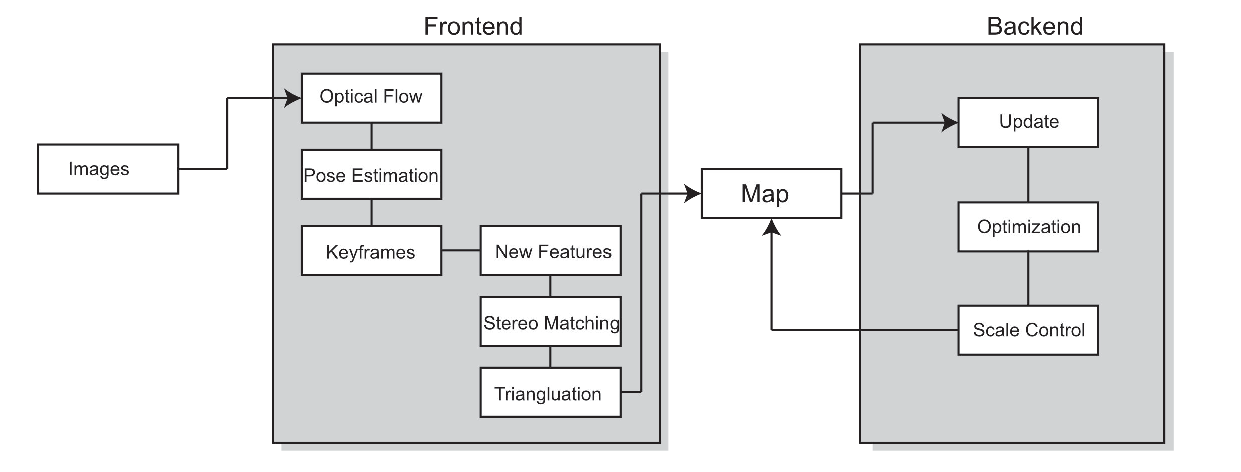
\includegraphics[width=1.0\linewidth]{designVO/pipeline.pdf}
	\caption{Processing pipeline.}
	\label{fig:pipeline}
\end{figure}

In this way, we have determined the general system flow, which will help the subsequent coding realization. Of course, in addition to the core algorithm, we also need some small peripheral modules to make the system more convenient, such as:
\begin{itemize}
	\item We should have a camera class to manage the intrinsic and extrinsics as well as the projection functions.
	\item We need a configuration file management class to facilitate reading content from configuration files. Some critical parameters can be store in the configuration file for quick debugging;
	\item Because the algorithm runs on the Kitti dataset, we need to read the image data according to Kitti's storage format, which should also be handled by a separate class.
	\item We need a visualization module to observe the running status of the system. Otherwise, we have to scratch our heads against a series of numeric values.
\end{itemize}

Although these modules are not the core parts, they are indispensable for implementation. Due to space limitations, we leave the peripheral code to readers.

\section{Implementation}
\subsection{Implement the Basic Data Structure}
Let's first implement the frame, feature, and landmark classes. It is usually recommended to set them as structs without defining complex private variables and interfaces. Considering that these data may be accessed and modified by multiple threads, we need to set thread locks in those parts.

The frame struct is:
\begin{lstlisting}[language=c++,caption=slambook2/ch13/include/myslam/frame.h]
struct Frame {
public:
	EIGEN_MAKE_ALIGNED_OPERATOR_NEW;
	typedef std::shared_ptr<Frame> Ptr;
	
	unsigned long id_ = 0;           // id of this frame
	unsigned long keyframe_id_ = 0;  // id of keyframe
	bool is_keyframe_ = false;       // keyframe?
	double time_stamp_;              // timestamp, not used in Kitti
	SE3 pose_;                       // pose defined as Tcw
	std::mutex pose_mutex_;          // Pose data mutex
	cv::Mat left_img_, right_img_;   // stereo images
	
	// extracted features in left image
	std::vector<std::shared_ptr<Feature>> features_left_;
	// corresponding features in right image, set to nullptr if no corresponding
	std::vector<std::shared_ptr<Feature>> features_right_;
	
public:  // data members
	Frame() {}
	
	Frame(long id, double time_stamp, const SE3 &pose, const Mat &left,
		const Mat &right);
	
	// set and get pose, thread safe
	SE3 Pose() {
		std::unique_lock<std::mutex> lck(pose_mutex_);
		return pose_;
	}
	
	void SetPose(const SE3 &pose) {
		std::unique_lock<std::mutex> lck(pose_mutex_);
		pose_ = pose;
	}
	
	/// Set keyframe and keyframe_id 
	void SetKeyFrame();
	
	/// create new frame and allocate id
	static std::shared_ptr<Frame> CreateFrame();
};
\end{lstlisting}

We define the frame struct to contain id, pose, image, and features in the left and right images. Among them, the pose will be set or accessed by the front and backends simultaneously, so we define its set and get functions and lock the data in them. Meanwhile, a frame can be constructed by a static function, and we can automatically set its id in the static create function.

Next, the feature struct:
\begin{lstlisting}[language=c++,caption=slambook2/ch13/include/myslam/feature.h]
struct Feature {
	EIGEN_MAKE_ALIGNED_OPERATOR_NEW;
	typedef std::shared_ptr<Feature> Ptr;
	
	std::weak_ptr<Frame> frame_;         // the frame that takes this feature
	cv::KeyPoint position_;              // 2D pixel position
	std::weak_ptr<MapPoint> map_point_;  // assigned map point
	
	bool is_outlier_ = false;       // is outlier?
	bool is_on_left_image_ = true;  // is detected on the left image?
	
	Feature() {}
	
	Feature(std::shared_ptr<Frame> frame, const cv::KeyPoint &kp)
		: frame_(frame), position_(kp) {}
};
\end{lstlisting}

The feature's main information is its 2D position and several flags describing whether it is an abnormal point and whether it is extracted in the left camera. We can access the host frame and its corresponding map point through a feature object. However, the real ownership of frame and map point objects belongs to the map. In order to avoid the circular reference generated by shared\_ptr, the weak\_ptr is used here \footnote{In short, the frame holds the shared\_ptr of feature, so we should avoid the feature holding frame's shared\_ptr again. Otherwise, the two structs refer to each other, which will cause the smart pointer to fail to be automatically destructed. }.

Finally the map point, or the landmark:
\begin{lstlisting}[language=c++,caption=slambook2/ch13/include/myslam/mappoint.h]
struct MapPoint {
	EIGEN_MAKE_ALIGNED_OPERATOR_NEW;
	typedef std::shared_ptr<MapPoint> Ptr;
	unsigned long id_ = 0;  // ID
	bool is_outlier_ = false;
	Vec3 pos_ = Vec3::Zero();  // Position in world
	std::mutex data_mutex_;
	int observed_times_ = 0;  // being observed by feature matching algo.
	std::list<std::weak_ptr<Feature>> observations_;
	
	MapPoint() {}
	
	MapPoint(long id, Vec3 position);
	
	Vec3 Pos() {
		std::unique_lock<std::mutex> lck(data_mutex_);
		return pos_;
	}
	
	void SetPos(const Vec3 &pos) {
		std::unique_lock<std::mutex> lck(data_mutex_);
		pos_ = pos;
	};
	
	void AddObservation(std::shared_ptr<Feature> feature) {
		std::unique_lock<std::mutex> lck(data_mutex_);
		observations_.push_back(feature);
		observed_times_++;
	}
	
	void RemoveObservation(std::shared_ptr<Feature> feat);
	
	std::list<std::weak_ptr<Feature>> GetObs() {
		std::unique_lock<std::mutex> lck(data_mutex_);
		return observations_;
	}
	
	// factory function
	static MapPoint::Ptr CreateNewMappoint();
};
\end{lstlisting}

The most important thing about MapPoint is its 3D position, which is the pos\_ variable, also needs to be locked. Its observation\_ variable records the features that observed this map point. Because the feature may be judged as an outlier, it needs to be locked when the observation part is changed.

So far, we have realized the basic data structure. In the framework, we let the map class actually hold these frame and map point objects, so we also need to define a map class:

\begin{lstlisting}[language=c++,caption=slambook2/ch13/include/myslam/map.h]
class Map {
public:
	EIGEN_MAKE_ALIGNED_OPERATOR_NEW;
	typedef std::shared_ptr<Map> Ptr;
	typedef std::unordered_map<unsigned long, MapPoint::Ptr> LandmarksType;
	typedef std::unordered_map<unsigned long, Frame::Ptr> KeyframesType;
	
	Map() {}
	
	void InsertKeyFrame(Frame::Ptr frame);
	
	void InsertMapPoint(MapPoint::Ptr map_point);
	
	LandmarksType GetAllMapPoints() {
		std::unique_lock<std::mutex> lck(data_mutex_);
		return landmarks_;
	}

	KeyframesType GetAllKeyFrames() {
		std::unique_lock<std::mutex> lck(data_mutex_);
		return keyframes_;
	}
	
	LandmarksType GetActiveMapPoints() {
		std::unique_lock<std::mutex> lck(data_mutex_);
		return active_landmarks_;
	}
	
	KeyframesType GetActiveKeyFrames() {
		std::unique_lock<std::mutex> lck(data_mutex_);
		return active_keyframes_;
	}
	
	void CleanMap();
	
private:

	void RemoveOldKeyframe();
	
	std::mutex data_mutex_;
	LandmarksType landmarks_;         // all landmarks
	LandmarksType active_landmarks_;  // active landmarks
	KeyframesType keyframes_;         // all keyframes
	KeyframesType active_keyframes_;  // active keyframes
	
	Frame::Ptr current_frame_ = nullptr;
	
	// settings
	int num_active_keyframes_ = 7;  
};
\end{lstlisting}
The map stores all keyframes and corresponding landmarks in a hash form and maintains an activated keyframe and map point set. Here the concept of activation is what we call the sliding window before. The backend will optimize the activated keyframes and landmark points and fix the rest to control the optimization scale. Of course, the activation strategy is defined by ourselves. The simple activation strategy is to remove the oldest keyframe and keep the latest keyframes in time. We only keep the latest 7 keyframes in this demo.

\subsection{Implement the Frontend}
After defining the basic data structure, let's consider the frontend functions. The frontend needs to determine the frame's pose based on the binocular image, but there are many alternative implementation choices. For example, how should we use the right eye's image? Do we track the feature in both left and right eyes or just one of them? When computing triangulation, should we consider the left and right images in the same frame or chronological order? In fact, any two images can be triangulated (for example, the left image of the previous frame vs. the right image of the next frame), so everyone's realization will be different.

For simplicity, we first determine the frontend processing logic:
\begin{enumerate}
	\item The frontend has three states: \textit{initialization}, \textit{normal tracking}, and \textit{tracking lost}.
	\item In the initialization state, we do the triangulation according to the optical flow matching between the left and right eyes. We will establish the initial map when successful.
	\item In the tracking phase, the front end calculates the optical flow from the previous frame to the current frame and estimates the image pose based on the optical flow result. This optical flow is used only for the left eye image to save the computation resource.
	\item If the tracked features are fewer than a threshold, we set the current frame as a keyframe. For keyframes, do the following things:
	
	\begin{itemize}
		\item Extract new feature points;
		\item Find the corresponding points of these points on the right, and use triangulation to create new landmarks;
		\item Add new keyframes and landmarks to the map and trigger a backend optimization.
		\item If the tracking is lost, reset the frontend system and reinitialize it.
	\end{itemize}
\end{enumerate}

According to this logic, the frontend processing flow is written as follows:
\begin{lstlisting}[language=c++,caption=slambook2/ch13/src/frontend.cpp]
bool Frontend::AddFrame(myslam::Frame::Ptr frame) {
	current_frame_ = frame;
	switch (status_) {
		case FrontendStatus::INITING:
			StereoInit();
			break;
		case FrontendStatus::TRACKING_GOOD:
		case FrontendStatus::TRACKING_BAD:
			Track();
			break;
		case FrontendStatus::LOST:
			Reset();
			break;
	}
	
	last_frame_ = current_frame_;
	return true;
}
\end{lstlisting}

The \textit{Track()} is implemented as:
\begin{lstlisting}[language=c++,caption=slambook2/ch13/src/frontend.cpp]
bool Frontend::Track() {
	if (last_frame_) {
		current_frame_->SetPose(relative_motion_ * last_frame_->Pose());
	}
	
	int num_track_last = TrackLastFrame();
	tracking_inliers_ = EstimateCurrentPose();
	
	if (tracking_inliers_ > num_features_tracking_) {
		// tracking good
		status_ = FrontendStatus::TRACKING_GOOD;
	} else if (tracking_inliers_ > num_features_tracking_bad_) {
		// tracking bad
		status_ = FrontendStatus::TRACKING_BAD;
	} else {
		// lost
		status_ = FrontendStatus::LOST;
	}
	
	InsertKeyframe();
	relative_motion_ = current_frame_->Pose() * last_frame_->Pose().inverse();
	
	if (viewer_) viewer_->AddCurrentFrame(current_frame_);
	return true;
}
\end{lstlisting}

In the \textit{TrackLastFrame()}, we call the optical flow of OpenCV to track the feature points:
\begin{lstlisting}[language=c++,caption=slambook2/ch13/src/frontend.cpp]
int Frontend::TrackLastFrame() {
	// use LK flow to estimate points in the right image
	std::vector<cv::Point2f> kps_last, kps_current;
	for (auto &kp : last_frame_->features_left_) {
		if (kp->map_point_.lock()) {
			// use project point
			auto mp = kp->map_point_.lock();
			auto px =
			camera_left_->world2pixel(mp->pos_, current_frame_->Pose());
			kps_last.push_back(kp->position_.pt);
			kps_current.push_back(cv::Point2f(px[0], px[1]));
		} else {
			kps_last.push_back(kp->position_.pt);
			kps_current.push_back(kp->position_.pt);
		}
	}
	
	std::vector<uchar> status;
	Mat error;
	cv::calcOpticalFlowPyrLK(
	last_frame_->left_img_, current_frame_->left_img_, kps_last,
	kps_current, status, error, cv::Size(21, 21), 3,
	cv::TermCriteria(cv::TermCriteria::COUNT + cv::TermCriteria::EPS, 30, 0.01),
	cv::OPTFLOW_USE_INITIAL_FLOW);
	
	int num_good_pts = 0;
	
	for (size_t i = 0; i < status.size(); ++i) {
		if (status[i]) {
			cv::KeyPoint kp(kps_current[i], 7);
			Feature::Ptr feature(new Feature(current_frame_, kp));
			feature->map_point_ = last_frame_->features_left_[i]->map_point_;
			current_frame_->features_left_.push_back(feature);
			num_good_pts++;
		}
	}
	
	LOG(INFO) << "Find " << num_good_pts << " in the last image.";
	return num_good_pts;
}
\end{lstlisting}

In the implementation, we often split the complex functions into some short functions until the underlying functions call OpenCV or g2o to achieve specific calculations. The readability and reusability of the program can be improved in this way. For example, the same feature extraction function can be used for both the initialization phase and the keyframe's new feature detection part. We recommend that readers go through this code by themselves (the frontend is less than 400 lines).

\subsection{Implement the Backend}
Compared with the frontend, the logic of the backend implementation will be more complicated. The overall backend implementation is as follows:
\begin{lstlisting}[language=c++,caption=slambook2/ch13/include/myslam/backend.h]
class Backend {
public:
	EIGEN_MAKE_ALIGNED_OPERATOR_NEW;
	typedef std::shared_ptr<Backend> Ptr;
	
	/// Start the backend thread in the constructor 
	Backend();
	
	// Set cameras and fetch the params
	void SetCameras(Camera::Ptr left, Camera::Ptr right) {
		cam_left_ = left;
		cam_right_ = right;
	}

	void SetMap(std::shared_ptr<Map> map) { map_ = map; }
	
	/// optimize and update the map
	void UpdateMap();
	
	/// stop the backend
	void Stop();
	
private:
	/// backend thread
	void BackendLoop();
	
	/// optimize the sliding window
	void Optimize(Map::KeyframesType& keyframes, Map::LandmarksType& landmarks);
	
	std::shared_ptr<Map> map_;
	std::thread backend_thread_;
	std::mutex data_mutex_;
	
	std::condition_variable map_update_;
	std::atomic<bool> backend_running_;
	
	Camera::Ptr cam_left_ = nullptr, cam_right_ = nullptr;
};
\end{lstlisting}

After the backend is started, it will wait for the condition variable of map\_update\_. When the map update is triggered, take the activated keyframes and map points from the map and perform optimization:
\begin{lstlisting}[language=c++,caption=slambook2/ch13/src/backend.cpp]
void Backend::BackendLoop() {
	while (backend_running_.load()) {
		std::unique_lock<std::mutex> lock(data_mutex_);
		map_update_.wait(lock);
		
		/// optimize the active frames and landmarks
		Map::KeyframesType active_kfs = map_->GetActiveKeyFrames();
		Map::LandmarksType active_landmarks = map_->GetActiveMapPoints();
		Optimize(active_kfs, active_landmarks);
	}
}
\end{lstlisting}

The optimization function is similar to the BA we used before, except that the data needs to be obtained from the frame and map point objects:
\begin{lstlisting}[language=c++,caption=slambook2/ch13/src/backend.cpp]
void Backend::Optimize(Map::KeyframesType &keyframes,
Map::LandmarksType &landmarks) {
	// setup g2o
	typedef g2o::BlockSolver_6_3 BlockSolverType;
	typedef g2o::LinearSolverCSparse<BlockSolverType::PoseMatrixType>
	LinearSolverType;
	auto solver = new g2o::OptimizationAlgorithmLevenberg(
	g2o::make_unique<BlockSolverType>(
	g2o::make_unique<LinearSolverType>()));
	g2o::SparseOptimizer optimizer;
	optimizer.setAlgorithm(solver);
	
	// pose vertices, use keyframe id
	std::map<unsigned long, VertexPose *> vertices;
	unsigned long max_kf_id = 0;
	for (auto &keyframe : keyframes) {
		auto kf = keyframe.second;
		VertexPose *vertex_pose = new VertexPose();  // camera vertex_pose
		vertex_pose->setId(kf->keyframe_id_);
		vertex_pose->setEstimate(kf->Pose());
		optimizer.addVertex(vertex_pose);
		if (kf->keyframe_id_ > max_kf_id) {
			max_kf_id = kf->keyframe_id_;
		}
		
		vertices.insert({kf->keyframe_id_, vertex_pose});
	}
	
	// landmark vertices, use landmark id
	std::map<unsigned long, VertexXYZ *> vertices_landmarks;
	
	// K and extrinsics
	Mat33 K = cam_left_->K();
	SE3 left_ext = cam_left_->pose();
	SE3 right_ext = cam_right_->pose();
	
	// edges
	int index = 1;
	double chi2_th = 5.991;  // robust kernel th
	std::map<EdgeProjection *, Feature::Ptr> edges_and_features;
	
	for (auto &landmark : landmarks) {
		if (landmark.second->is_outlier_) continue;
		unsigned long landmark_id = landmark.second->id_;
		auto observations = landmark.second->GetObs();
		for (auto &obs : observations) {
			if (obs.lock() == nullptr) continue;
			auto feat = obs.lock();
			if (feat->is_outlier_ || feat->frame_.lock() == nullptr) continue;
			
			auto frame = feat->frame_.lock();
			EdgeProjection *edge = nullptr;
			if (feat->is_on_left_image_) {
				edge = new EdgeProjection(K, left_ext);
			} else {
				edge = new EdgeProjection(K, right_ext);
			}
			
			// add landmark verices if not contained
			if (vertices_landmarks.find(landmark_id) ==
				vertices_landmarks.end()) {
				VertexXYZ *v = new VertexXYZ;
				v->setEstimate(landmark.second->Pos());
				v->setId(landmark_id + max_kf_id + 1);
				v->setMarginalized(true);
				vertices_landmarks.insert({landmark_id, v});
				optimizer.addVertex(v);
			}
			
			edge->setId(index);
			edge->setVertex(0, vertices.at(frame->keyframe_id_));    // pose
			edge->setVertex(1, vertices_landmarks.at(landmark_id));  // landmark
			edge->setMeasurement(toVec2(feat->position_.pt));
			edge->setInformation(Mat22::Identity());
			auto rk = new g2o::RobustKernelHuber();
			rk->setDelta(chi2_th);
			edge->setRobustKernel(rk);
			edges_and_features.insert({edge, feat});
			
			optimizer.addEdge(edge);
			
			index++;
		}
	}
	
	// do optimization and eliminate the outliers
	optimizer.initializeOptimization();
	optimizer.optimize(10);
	
	int cnt_outlier = 0, cnt_inlier = 0;
	int iteration = 0;
	while (iteration < 5) {
		cnt_outlier = 0;
		cnt_inlier = 0;
		// determine if we want to adjust the outlier threshold
		for (auto &ef : edges_and_features) {
			if (ef.first->chi2() > chi2_th) {
				cnt_outlier++;
			} else {
				cnt_inlier++;
			}
		}
		double inlier_ratio = cnt_inlier / double(cnt_inlier + cnt_outlier);
		if (inlier_ratio > 0.5) {
			break;
		} else {
			chi2_th *= 2;
			iteration++;
		}
	}
	
	for (auto &ef : edges_and_features) {
		if (ef.first->chi2() > chi2_th) {
			ef.second->is_outlier_ = true;
			// remove the observation
			ef.second->map_point_.lock()->RemoveObservation(ef.second);
		} else {
			ef.second->is_outlier_ = false;
		}
	}
	
	LOG(INFO) << "Outlier/Inlier in optimization: " << cnt_outlier << "/"
		<< cnt_inlier;
	
	// Set pose and lanrmark position
	for (auto &v : vertices) {
		keyframes.at(v.first)->SetPose(v.second->estimate());
	}
	for (auto &v : vertices_landmarks) {
		landmarks.at(v.first)->SetPos(v.second->estimate());
	}
}
\end{lstlisting}

The back end is shorter than the front end, with less than 200 lines.

\section{Experiment Results}
Finally, we look at the running effect of this visual odometry. First, we need to download the Kitti dataset from \url{http://www.cvlibs.net/datasets/kitti/eval_odometry.php}. Its odometry data is about 22GB. After downloading, we decompress it and get several video segments. Let's take segment 0 as an example. After compiling the program in this section, fill in the path corresponding to the configuration file config/default.yaml. In my machine, it looks like this:
$$\text{dataset_dir: /media/xiang/Data/Dataset/Kitti/dataset/sequences/00}.$$

Then we run it with:
\begin{lstlisting}[language=sh,caption=Terminal input:]
bin/run_kitti_stereo
\end{lstlisting}
Then you can see the SLAM output, as shown in \autoref{fig:snapshot-vo}. During operation, the program will display the activated keyframes and maps, which should continue to grow and disappear as the camera moves.

\begin{figure}[!htp]
	\centering    
	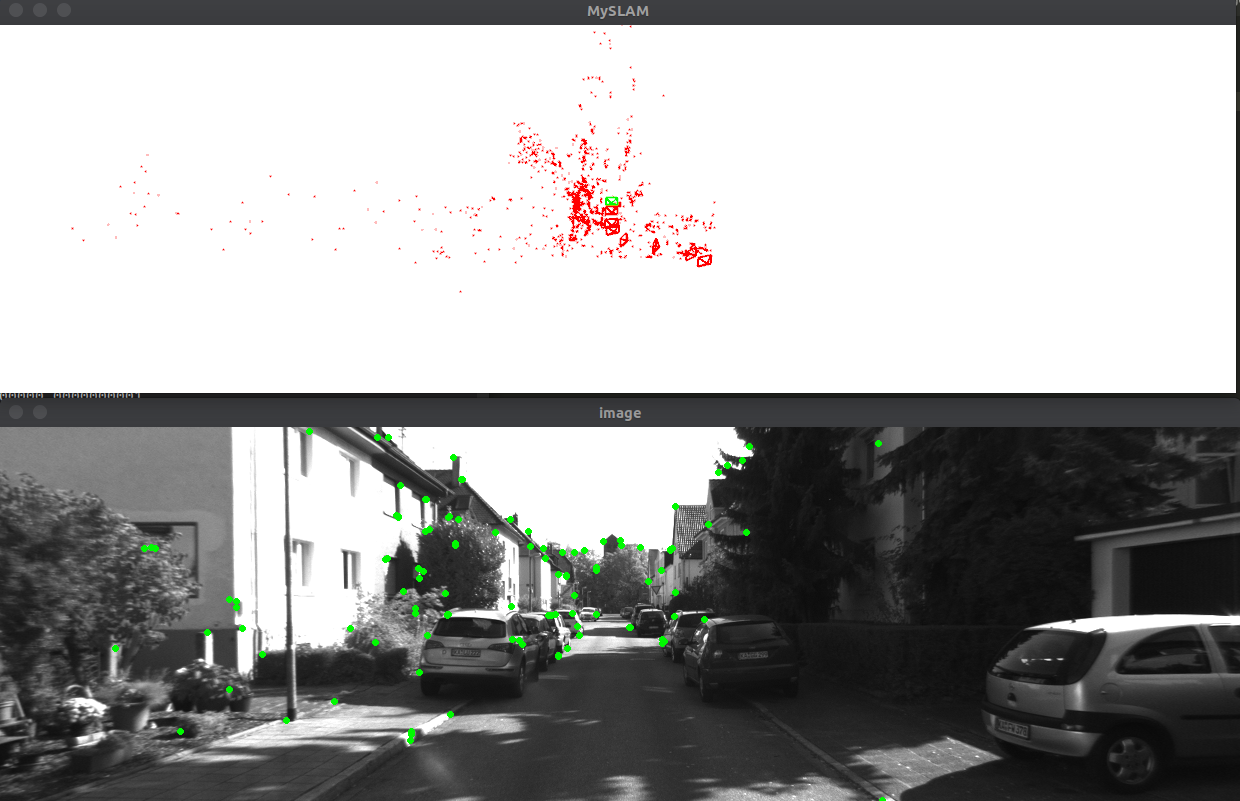
\includegraphics[width=0.9\linewidth]{designVO/snapshot-vo.png}\\
	\caption{Snapshot of the visual odometry.}
	\label{fig:snapshot-vo}
\end{figure}

We print the run time it takes for a single frame. When dealing with non-keyframes, the time is about 16ms. When processing keyframes, the time-consuming will increase due to the additional steps of extracting features and the right eye matching. Moreover, since our map currently stores all keyframes and map points, it will cause memory growth after running for a while. If readers do not need all maps, they can keep only the active part.

\section*{Exercises}
\begin{enumerate}
	\item Do you understand all the C++ techniques used in this book? If there is something you are not familiar with, use search engines to learn the related knowledge, including range-based for loops, smart pointers, singleton patterns in design patterns, threads and locks, and so on.
	\item Consider optimizing the system introduced in this lecture. For example, use a faster method of extracting feature points (this demo uses GFTT, which is not fast), use a 1-d search instead of 2d optical flow when matching left and right images, and use the direct method to estimate the pose and features at the same time, etc.
	\item* Add a loop detection thread to the demo, and use a pose graph to optimize when a loop is detected to eliminate accumulated errors.
\end{enumerate}


